%  --------------------------------------------------------------------------
%  IPA Qualitätssicherung für Djangoprojekte Dokumentation
%  Created by Vladimir Kuzma on 2012-04-30.
%  --------------------------------------------------------------------------

%  --------------------------------------------------------------------------
%  Latex Document Settings
%  --------------------------------------------------------------------------

\documentclass[
11pt, % Schriftgrösse
a4paper, % A4 Papier
BCOR10mm, % Absoluter Wert der Bindekorrektur, z.B. BCOR1cm
DIV14, % Satzspiegel festlegen siehe
       % http://www.ctex.org/documents/packages/nonstd/koma-script.pdf
footsepline = false, % Trennlinie zwischen Textkörper und Fußzeile
                     % bei normalen Seiten
headsepline, % Trennlinie zwischen Kopfzeile und Textkörper
             % bei normalen Seiten
oneside, % Zweiseitig
openright,
halfparskip, % Europäischer Satz mit Abstand zwischen den Absätzen
abstracton, % inkl. Abstract
listof=totocnumbered, % Abb.- und Tab.verzeichnis im Inhaltsverzeichnis
bibliography=totocnumbered % Lit.zeichnis in Inhaltsverzeichnis aufnehmen
]{scrreprt}

\usepackage[automark]{scrpage2} % Gestaltung von kopf- und Fußzeile
\usepackage[ngerman]{babel}
\usepackage[ngerman]{translator}
\usepackage{tocbasic}
\usepackage[utf8]{inputenc}
\usepackage{lmodern} % Latin Modern
\usepackage[T1]{fontenc}
\usepackage{hyphenat}
\usepackage{ae} % Schöne Schriften für PDF-Dateien

% Tradmark
\def\TTra{\textsuperscript{\texttrademark}}

%1.5 Zeilenabstand
\usepackage[onehalfspacing]{setspace}

% Festlegung des Seitenstils (scrpage2)
\pagestyle{scrheadings}
\clearscrheadfoot
\automark[chapter]{section}

% \lehead{\sffamily\upshape\headmark}
% \cehead{}
% \rehead{}
% \lefoot[\pagemark]{\upshape \pagemark}
% \cefoot{}
% \refoot{}
% \lohead{}
% \cohead{}
\lohead{\sffamily\upshape\headmark}
\lofoot{}
\cofoot[\today]{\today}
\rofoot[\pagemark]{\scshape \pagemark}

% Surround parts of graphics with box
\usepackage{boxedminipage}

% Package for including code in the document
\usepackage{listings}

% If you want to generate a toc for each chapter (use with book)
\usepackage{minitoc}
\usepackage{longtable}

% Abkürzungsverzeichnis erstellen.
\usepackage[printonlyused]{acronym}

% schöne Tabelle zeichnen
\usepackage{booktabs}
\renewcommand{\arraystretch}{1.4} %Die Zeilenabstände in Tabellen angepasst.

% für variable Breiten
\usepackage{tabularx}

% Durchgestrichener Text
\usepackage[normalem]{ulem} %emphasize weiterhin kursiv

% This is now the recommended way for checking for PDFLaTeX:
\usepackage{ifpdf}

\usepackage{eurosym}

\usepackage{natbib}

\usepackage{paralist}

\usepackage{array,ragged2e}

\usepackage[hyperfootnotes=false]{hyperref}
\hypersetup{
  bookmarks=true,         % show bookmarks bar?
  unicode=true,           % non-Latin characters in Acrobat’s bookmarks
  pdftoolbar=true,        % show Acrobat’s toolbar?
  pdfmenubar=true,        % show Acrobat’s menu?
  pdffitwindow=true,      % window fit to page when opened
  pdfstartview={FitH},    % fits the width of the page to the window
  pdftitle={IPA Dokumentation},   
  pdfauthor={Marius Küng},
  pdfsubject={Dokumentation IPA yatplaner},
  pdfcreator={TeX Live 2009},
  pdfproducer={pdfTeX, Version 3.1415926-1.40.10},
  pdfnewwindow=true,      % links in new window
  colorlinks=true,       % false: boxed links; true: colored links
  linkcolor=black,          % color of internal links
  citecolor=black,        % color of links to bibliography
  filecolor=magenta,      % color of file links
  urlcolor=cyan          % color of external links
  % linkcolor=black,          % color of internal links
  % citecolor=black,        % color of links to bibliography
  % filecolor=black,      % color of file links
  % urlcolor=black          % color of external links
}

\ifpdf
    \usepackage[pdftex]{graphicx}
\else
    \usepackage{graphicx}
\fi

\makeatletter 
\let\orgdescriptionlabel\descriptionlabel 
\renewcommand*{\descriptionlabel}[1]{% 
  \let\orglabel\label 
  \let\label\@gobble 
  \phantomsection 
  \edef\@currentlabel{#1}% 
  %\edef\@currentlabelname{#1}% 
  \let\label\orglabel 
  \orgdescriptionlabel{#1}% 
} 
\makeatother 

%  --------------------------------------------------------------------------
%  Start Document
%  --------------------------------------------------------------------------
\title{Dokumentation IPA Qualitätssicherung für Djangoprojekte}

\author{IPA in Applikationsentwicklung\\
    \\
    Auszubildender - Vladimir Kuzma\\
	Auftraggeber - allink GmbH\\
    Projektleiter - Silvan Spross\\
    Experte - Roman Fischer\\
    Chefexperte -  \\
    Durchführungsort - allink GmbH\\
	\\
	Informatikschule ZLI }

\date{30.04. - 16.05.2012}

\begin{document}
    \ifpdf
        \DeclareGraphicsExtensions{.pdf, .jpg, .tif}
    \else
        \DeclareGraphicsExtensions{.eps, .jpg}
    \fi

    \pagenumbering{Alph}
  
    \maketitle

    \pagenumbering{arabic}
  
    \tableofcontents
    
    \part{Umfeld und Ablauf}
         \chapter{Aufgabenstellung}
             %!TEX root = ../dokumentation.tex
\section{Titel der Facharbeit} 
Kontinuierliche Qualitätssicherung für Web Projekte in Django
    
\section{Thematik}
Es soll eine Software in Python erstellt werden, welche kontinuierlich die Qualität von einer konfigurierbaren Menge Django Projekte überprüft.

\section{Klassierung}
    
\begin{itemize}
    \item Prozessautomatisierung 
    \item UNIX / Linux
    \item Python / Ruby
\end{itemize}
    
\section{Durchführungsblock}
Startblock 10: 16.04.2012 - 20.04.2012\\
IPA-Durchführung: 30.04.2012 - 16.05.2012\\
Einreichung bis: Montag, 16.03.2012\\
    
\section{Ausgangslage}
Bei allink besteht seit Mitte 2010 ein Entwicklungs- und Deployment-Prozess welcher sich in den letzten eineinhalb Jahren etabliert hat. Die Entwickler sparen sich dadurch pro Projekt einige Stunden Arbeit und die Projekte sind zudem auch nach längere Zeit noch wartbar. Dank der Abhängigkeitsdefinitionen pro Projekt, können Entwickler schnell in einem anderem Projekt einsteigen oder in einem alten Projekt Fehlerkorrekturen vornehmen. Seit einem halben Jahr wird zudem die Codequalität mit Hilfe von einer automatischen Überprüfung der Codekonvention auf den Rechnern der Entwickler erhöht.

Trotz all diesen Massnahmen ist es möglich, dass Entwickler ein Projekt unabsichtlich verunreinigen. Im Extremfall führt dies dazu, dass das Projekt bei einem anderen Entwickler oder sogar in der Produktion nicht mehr lauffähig ist.

Mit dieser Arbeit soll ein System zur automatischen Kontrolle der erwähnten Faktoren erstellt werden.

\section{Detaillierte Aufgabenstellung}
Es soll eine Software in Python erstellt werden, welche kontinuierlich die Qualität von einer konfigurierbaren Menge Django Projekte überprüft. Dazu sollen die Projekte jeweils täglich aus dem Versionierungssystem geklont, Projektspezifische Abhängigkeiten installiert und nach gewissen Anforderungen getestet und abschliessend ein projektübergreifender Report per E-Mail versendet werden.

Diese Anforderungen sind:

- Installierbarkeit der projektspezifischen Abhängigkeiten
Erklärung: Jedes Projekt hat projektspezifische Abhängigkeiten, welche sich über ein Packetmanagement installieren lassen. Bei dieser Anforderung soll pro Projekt geprüft werden, ob diese Abhängigkeitsliste komplett und korrekt ist.

- Codekonventionen nach PEP8
Erklärung: Im ''Python Enhancement Proposal 8'' sind die grundlegenden Stil-Richtlinien für Python-Quellcode definiert. Bei dieser Anforderung soll pro Projekt geprüft werden, dass diese Stil-Richtlinien eingehalten wurden.

- Überprüfung der Syntax
Erklärung: Überprüft werden sollen sämtliche Python und Javascript Files z.B. mit pyflakes und jshint.

- Initialisierung der Datenbank

- Durchführen sämtlicher Datenbankmigrations-Files

- UnitTests

Treten bei den Tests Fehler auf, soll dies in einem E-Mail festgehalten und an eine Sammeladresse gesendet werden.

Eine weitere Anforderung an die Software ist, dass die einzelnen Überprüfungen der Anforderungen Modular aufgebaut sind und so in Zukunft weitere Anforderungen hinzugefügt werden können. Zudem kommt hinzu, dass die neu zu schreibende Applikation mit dem Versionsverwaltungssystem git verwaltet werden soll. Dabei sollen zwei Branches geführt werden: ''develop'' und ''master''. Wobei der ''master'' immer den Stand der Produktion widerspiegelt und im ''develop'' weiterentwickelt wird.

Es sollen wo möglich bestehende Tools zur Überprüfung der oben genannten Anforderungen verwendet werden. Dies bedeutet für den Lernenden, dass er überwiegend die Software zum Koordinieren und zusammenführen der einzelnen Tests schreiben muss.

Nicht Bestandteil dieser Arbeit sind:

- VirtualMachine zur Entwicklung
- Bereitstellung des Zielsystems
- Einpflegen aller Projekte

Nebst der begleitenden IPA Dokumentation wird keine zusätzliche Dokumentation gefordert.

\section{Mittel und Methoden}
Folgende Technologien sind zwingend zu verwenden:

\begin{itemize}
    \item  Python 2.x
    \item  Django
\end{itemize}

Der Lernende muss sich zudem während der Entwicklung an die Firmenstandards halten, welche im IT Wiki zugänglich sind.
    
\section{Vorkenntnisse}
Dem Lernenden sind alle genannten Technologien bereits bekannt. Seit Beginn seines Praktikums im Mai 2010 setzt er sich damit auseinander.
    
\section{Vorarbeiten}
Die Testumgebung wird als VirtualMachine Image mit einem unserem Produktivsystem am nächsten kommenden System bespielt und dem Lernenden zur Verfügung gestellt.    

\section{Neue Lerninhalte}
Wie erwähnt sind dem Lernenden alle Technologien bereits bekannt. Das Know-how ist zudem bei allink ausreichend vorhanden. 

\section{Arbeiten in den letzten 6 Monaten}
Der Lernende hat diverse Webseiten mit den oben genannten Technologien umgesetzt.

        \chapter{Einleitung}
            %!TEX root = ../dokumentation.tex
\section{Projekorganisation}

\begin{figure}[!ht]
\begin{center}
    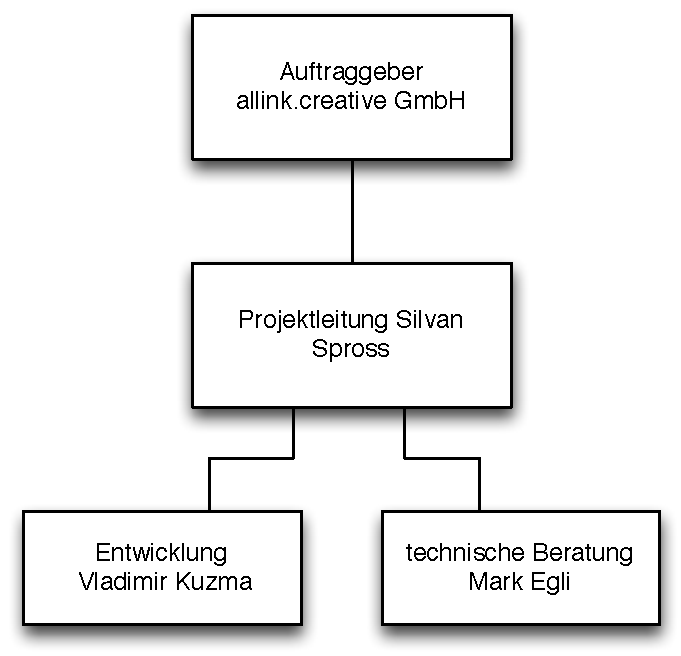
\includegraphics[width=0.5\textwidth,angle=0]{./grafiken/organigram.pdf}
\end{center}
\end{figure}
\footnotetext{Eigene Darstellung}

\section{Projektbeschreibung}
Es soll eine Software in Python erstellt werden, welche kontinuierlich die Qualität von einer konfigurierbaren Menge Django Projekte überprüft. Dazu sollen die Projekte jeweils täglich aus dem Versionierungssystem geklont, Projektspezifische Abhängigkeiten installiert und nach gewissen Anforderungen getestet und abschliessend ein projektübergreifender Report per E-Mail versendet werden.

\section{Rahmenbedingung}
Die Anwendung soll mit folgenden Mitteln realisiert werden:

Technologien
\begin{itemize}
    \item Python 

\end{itemize}

Anwendungen
\begin{itemize}
    \item pep8
    \item pyflakes
    \item jshint
\end{itemize}

Systemen
\begin{itemize}
    \item Mac OS X
    \item Debian lenny
\end{itemize}
    
\section{Systemumgebung}
\begin{itemize}
    \item Betriebsystem (Projekumsetzung): Mac OS X
    \item Editor: vim
    \item Dokumentationshilfsmittel: LaTeX
    \item Entwicklungsumgebung: Python
    \item localer Testserver: Debian Server in einer VM (Virtualbox) 
    \item Versionierung: Git, auf Github veröffentlicht
\end{itemize}

\section{Projektplannungsmethode}
Ich habe mich für die Projektplanungsmethode IPERKA entschieden. \\

\subsection{Begründung}
Für ein kleines Projekt reicht IPERKA meiner Meinung ausreichend aus. Die Planungs- und die Realisierungsphase ist klar getrennt. Es sind alle wichtigen Arbeitsschritte vorhanden, die eine saubere Struktur und ausführliche Dokumentation erlauben. 

\clearpage

        \chapter{Projektplanung}
            \input{./kapitel/03_projektplanung.tex}
    % \part{Projekt}
    %     \chapter{Projektbeschreibung}
    %         \input{./kapitel/04_projektbeschreibung.tex}
    %     \chapter{Realisierung}
    %         \input{./kapitel/05_realisierung.tex}
    %     \chapter{Testing}
    %         \input{./kapitel/06_testing.tex}
    %     \chapter{Konklusion}
    %         \input{./kapitel/07_konklusion.tex}

    
    \appendix
    
    \listoffigures
    \listoftables
    % 
    % \chapter{Abkürzungsverzeichnis}
    %     \input{./kapitel/09_acronym.tex}
    % \lstlistoflistings
  
    \bibliographystyle{unsrtnat}
    \bibliography{literaturverzeichnis}
    
    % \chapter{Literaturverzeichnis}
    %     \input{./kapitel/08_quellen.tex}
    % 
    % \chapter{Arbeitsjournal}
    %     \input{../arbeitsjournal/arbeitsjournal.tex}
    
\end{document}
